%%%%%%%%%%%%%%%%%%%%%%%%%%%%%%%%%%%%%%%%%%%%%%%%%%%%%% SETTINGS %%%%%%%%%%%%%%%%%%%%%%%%%%%%%%%%%%%%%%%%%%%%%%%%%%%%%%%%%%%%%
%clear; bibtex main.aux;pdflatex main.tex ;evince main.pdf &

\documentclass[final,12pt]{report} 						% list options between brackets [draft]

\pdfminorversion = 5									% changing the default PDF version

\usepackage[utf8]{inputenc}								% list packages between braces
\usepackage{graphicx,keystroke}							% colors, scaling and rotation of EPS files (convert file.jpeg file.eps)
\usepackage[frenchb]{babel}								% french as main language
\usepackage[left=0.80in, right=0.80in, top=1.0in, bottom=1.0in]{geometry}		% define margin
\usepackage{verbatim} 									% LaTeX multiline comments
\usepackage{subfig}										% Enable sub figures
\usepackage{amsmath,epsfig}								% Formula
\usepackage[T1]{fontenc}								% pipe... symbol
\usepackage{fancyhdr}									% header, footer
\usepackage{hyperref}									% URL
\usepackage[hyperpageref]{backref}						% Adds ‘backlink’ text to the end of each item in the bibliography
\usepackage{natbib}										% Reimplement the LATEX \cite command
\usepackage{amssymb}									% American Mathematical Society symbol Real En	
\usepackage[toc,page,titletoc]{appendix}				% 
\usepackage[toc,xindy]{glossaries}						% Use glossaries


%\usepackage{multirow}									% tabular addition
%\usepackage{normalem}									% Overwrite \emph and permit barred text, special underlining...

%\usepackage{tikz}
%\usepackage{kpfonts}
%\usepackage[explicit]{titlesec}

								% Custom packages		

\makeatletter

\renewcommand{\maketitle}{%
{
	\pagestyle{empty}
\begin{center}

	\href{http://www.istia.univ-angers.fr}{
\includegraphics[width=5cm]{figure/logo_univ_angers.png}}\\
	\bigskip
	
	\begin{LARGE}
		Master Recherche Mathématiques et Applications\\
		%Master Recherche en Systèmes Dynamiques et Signaux\\
	\end{LARGE}\bigskip
	
	\begin{large}
		Spécialité : S\textsc{ystèmes} D\textsc{ynamiques et} S\textsc{ignaux}\\
		%Année 2010-2011\\
	\end{large}\bigskip\bigskip
	
%	\begin{LARGE}
%		Rapport bibliographique intermédiaire\\% de Master 2 Recherche SDS:\\
%	\end{LARGE}\bigskip
	
	\begin{large}
		Soutenu par : \href{http://www.christophe-rigaud.com}{Christophe RIGAUD}\\
	\end{large}\bigskip\bigskip

	\begin{normalsize}
		le 7 juillet 2011\\
	\end{normalsize}\medskip
	
	\begin{normalsize}
		Au sein de l'Institut des Sciences et Techniques de l'Ingénieur d'Angers\\
		%LISA - ISTIA - 62 avenue Notre-Dame du Lac 49000 ANGERS\\\bigskip
		\bigskip\bigskip\bigskip
	\end{normalsize}
	
	\begin{Large}
		\bf{Interprétation d'images et graphe conceptuel intégrant des connaissances topologiques et photométriques}
		\bigskip\bigskip\bigskip
	\end{Large}
	
	\begin{normalsize}
		Jury:\\
	\end{normalsize}
	\parbox{15cm}{
		\begin{tabbing}
			Président :\hspace{4em}\= L. Hardouin\hspace{5em}\= Professeur Université d'Angers\\
			Examinateurs :   	\> L. Autrique	\> Professeur Université d'Angers\\
				\> F. Chapeau Blondeau	\> Professeur Université d'Angers\\
				\> J.L. Boimond			\> Professeur Université d'Angers\\
				%\> M. Bourcerie			\> Professeur Université d'Angers\\
				%\> P. Declerck			\> MCF Université d'Angers\\
				\> J.B. Fasquel  		\> MCF Université d'Angers\\
				\> C. Jean-Guillaume	\> MCF Université d'Angers\\
				\> M. Lhommeau			\> MCF Université d'Angers\\
				\> D.Rousseau			\> MCF Université d'Angers
		
		\end{tabbing}
	}
	\bigskip\bigskip\bigskip
\end{center}
	\begin{large}
		Encadrant: Jean-Baptiste FASQUEL		
	\end{large}
	\begin{flushright}
	\parbox{15cm}{
		\begin{flushright}

		
\includegraphics[width=4cm]{figure/logo_lisa.png}

		LABORATOIRE D’INGÉNIERIE DES SYSTÈMES AUTOMATISÉS 

		EA 4094 - Université d’Angers
		\end{flushright}}
		\end{flushright}
		\clearpage
	}
}

%\def\thechapter{\Roman{chapter}} 
%\def\thesection{\arabic{section}} 
        
% Chapter (general)
\def\@makechapterhead#1{%
  {\parindent \z@ \raggedright \normalfont
    \ifnum \c@secnumdepth >\m@ne
        %\huge\bfseries \@chapapp\space \thechapter
        \par\nobreak
        \vskip 20\p@
    \fi
    \interlinepenalty\@M
    \Huge \bfseries \thechapter \hspace{0.2em} #1 \par\nobreak
    \vskip 30\p@			% space under chapter name
  }}

% Chapter table of content
\def\@makeschapterhead#1{%
  {\parindent \z@ \raggedright
    \normalfont
    \interlinepenalty\@M
    \Huge \bfseries  #1\par\nobreak
    \vskip 40\p@			% space under "table of content"
  }}


\makeatother
								% Custom commands
%
%----------------------------------------------
%HEADER
\pagestyle{fancy}
\fancyhead{} 															% Clear all header fields
\fancyhead[RO,RE]{\includegraphics[height=30pt]{pic/pic\thepage.png}}	% Right Odd AND Right Even 
\fancyhead[LO,LE]{\rightmark}											% Left Odd AND Left Even

\fancyfoot{}															% Clear all foot fields
%\fancyfoot[L]{Christophe Rigaud}
\fancyfoot[C]{}
\fancyfoot[R]{\thepage}
%\fancyfoot[L]{\href{http://www.christophe-rigaud.com}{Christophe Rigaud}}

%----------------------------------------------
%LINK AND WINDOW
\hypersetup{
    colorlinks,
    citecolor=black,
    filecolor=black,
    linkcolor=black,
    urlcolor=black,
    unicode=false,          					% non-Latin characters in Acrobat’s bookmarks
    pdftoolbar=true,        					% show Acrobat’s toolbar?
    pdfmenubar=true,        					% show Acrobat’s menu?
    pdffitwindow=false,    						% window fit to page when opened
    pdfstartview={FitH},    					% fits the width of the page to the window
    pdftitle={Rapport de Master Recherche Mathématiques et Applications - Christophe Rigaud - 2011},    % title
    pdfauthor={Christophe Rigaud},     			% author
    pdfsubject={Interprétation d'images et graphe conceptuel intégrant des connaissances topologiques et photométriques},   			% subject of the document
    pdfcreator={Christophe Rigaud},   			% creator of the document
    pdfproducer={pdflatex}, 			% producer of the document
    pdfkeywords={Traitment d'image} {graphe conceptuel} {conceptuel} {topologie} {photométrie} {christophe rigaud}, % list of keywords
    pdfnewwindow=true      						% links in new window
}
%\hypersetup{
%	%DOC : http://www.tug.org/applications/hyperref/manual.html
%    %bookmarks=true,        % show bookmarks bar?
%    unicode=false,          % non-Latin characters in Acrobat’s bookmarks
%    pdftoolbar=true,        % show Acrobat’s toolbar?
%    pdfmenubar=true,        % show Acrobat’s menu?
%    pdffitwindow=false,     % window fit to page when opened
%    pdfstartview={FitH},    % fits the width of the page to the window
%    pdftitle={Rapport de Master - Christophe Rigaud},    % title
%    pdfauthor={Christophe Rigaud},     			% author
%    pdfsubject={Traitement d'image},   			% subject of the document
%    pdfcreator={Christophe Rigaud},   			% creator of the document
%    pdfproducer={Christophe Rigaud}, 			% producer of the document
%    pdfkeywords={image} {conceptuel} {méthode}, % list of keywords
%    pdfnewwindow=true,      % links in new window
%%    colorlinks=false,       % false: boxed links; true: colored links
%    linkcolor=black,          % color of internal links
%%    citecolor=green,        % color of links to bibliography
%%    filecolor=magenta,      % color of file links
%%    urlcolor=green          % color of external links
%}

%----------------------------------------------
% Document settings

%\setcounter{secnumdepth}{3} %subsubsections are numbered
%\setcounter{tocdepth}{3} %subsubsections are added to the TOC

%\renewcommand{\tocbibname}{References} 

\hyphenation{li-mi-terons i-ma-ges in-flu-ence}

%----------------------------------------------
%Alter page dimensions

%\setlength{\textwidth}{16cm}
%\setlength{\oddsidemargin}{0.46cm}
%\setlength{\evensidemargin}{0.46cm}
%\setlength{\textheight}{22.3cm}
%\setlength{\topmargin}{-0.54cm}
%\setlength{\headsep}{1.5cm}
%\setlength{\footnotesep}{0.6cm} 



									% Custom styles



%%%%%%%%%%%%%%%%%%%%%%%%%%%%%%%%%%%%%%%%%%%%%%%%%%%%%% DOCUMENT %%%%%%%%%%%%%%%%%%%%%%%%%%%%%%%%%%%%%%%%%%%%%%%%%%%%%%%%%%%%%

%\makeglossaries
%\newglossaryentry{ROI}{name={ROI}, description={app Domain Description...}}

%\newglossaryentry{sample}{name={has been inserted aaa},description={testing testing 123}}
%\newglossaryentry{topologie}{description={La topologie est une branche des mathématiques concernant l'étude des déformations spatiales par des transformations continues (sans arrachages ni recollement des structures)\url{http://fr.wikipedia.org/wiki/Topologie}}
%\newglossaryentry{Moteur d'inférence, de l'anglais "enference engine" et du verbe « inférer » qui signifie « déduire », c'est un concept de raisonnement déductif, qui peut être concrètement un logiciel, à qui on demande des informations et qui essaye de les déduire à partir de sa base de connaissances.})
%\footnote{Le fenêtrage est le fait de considérer qu'une fraction de la dynamique d'une image (exemple : un intervalle dans un histogramme d'image), on l'utilise souvent pour faciliter la visualisation ou les traitements d'une image.}

\begin{document}
	%--------------------------------------------------------------------------------------------------
	\renewcommand{\labelitemi}{$\bullet$}
	\renewcommand{\appendixtocname}{Annexes}
	\newcounter{ale}
	\setcounter{tocdepth}{4}



\chapter{Doctoral consortium application}

\section{General Information}
% \begin{tabular}{ l r  }
  \begin{tabular}{| p{4cm} | p{12.8cm} | }
\hline
      Name surname: & \href{http://www.christophe-rigaud.com/}{Christophe Rigaud} \\
\hline
      University: & Laboratory L3i, University of La Rochelle, France\\
\hline
%       Thematic axe & IDDC \\ \hline
%       Phone & +33 6 80 81 00 22 \\ \hline
%       Email & christophe.rigaud@univ-lr.fr \\ \hline
%       Web page & http://l3i.univ-larochelle.fr/Rigaud-Christophe.html \\  \hline
%       &  \\ \hline
%       End date & October 1st, 2014 \\ \hline
      Supervisors: & Jean-Christophe Burie, Dimosthenis Karatzas and Jean-Marc Ogier  \\ 
\hline
      Thesis title:&  Segmentation and indexation of complex object: application to the detection and recognition of complex objects in comics books\\
\hline
      Date:	&  October 1$^{st}$, 2011 to September 30$^{st}$, 2014 \\
\hline

%       Scholarship & Ministry \\ \hline
    \end{tabular}
%     & 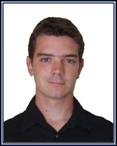
\includegraphics{fig/christophe_rigaud-ce168.jpg} \\
% \end{tabular}
% 	- your name and surname
% 	- advisor's names (mine is: Oriol Ramos Terrades)
% 	- thesis title
% 	- admission date

%-------------------------------------------------------------------------------------

\section{Research plan}
\subsection{Overview}
L3i lab initiated the e-BDthèque project to develop digital comics books under the CPER 2008-2013 founds. Nowadays, many large scale digitalization processes of comics are considered at national and international scale. From one hand, the digitalization of the comics rise new needs of indexing tools allowing to browse a large amount of data. With such tool, it could be possible to find specific drawings, animate objects or characters, analyse specific strip sequence, etc... On the other hand, several company feedbacks shows that there is no tool allowing to automatically extract comics content from digitized books such as frames, speech balloons and text. The implementation of reading scenario for new devices as tablet and smartphones is made manually and take an terrible time. The development of automatic content extraction tools is relevant for full-text search, frame per frame reading, automatic translation, text-to-speech, etc...


%Image processing has been widely studied during the last decades on grey-scale image and on colour images. We are now able to provide a low level description for simple object recognition purpose. In the case of complex object composed of many regions as comics characters (where each region has its own shape, colour, texture), it is necessary to consider the location of each region as well. A priori model of character is very tricky to specify because of shadow, posture and overlapping variabilities.
%This thesis focus on, from one hand, frame-content description, and on another hand, to propose an indexation process with the objective of redundant structure retrieval among the different frames of the comics albums. These particular structures may be assimilated as recurrent object and therefore characters or special sceneries.
 %The user may be included in the loop to interact throughout the process and provide relevant feedback to revise the description model in order to reach a ``high level'' description.
%The last step is passing from ``high level'' (e.g. it is a character) to semantic representation (e.g. it is Tintin/Asterix). This representation will enrich a system of knowledge representation developed as part of another thesis.

\subsection{Contributions}
Comics content many heterogeneous elements that is better to treat separately. We decided to split our work into several steps. First, we defined a dataset and its ground truth in order to evaluate our work later on and to share with the community, make new cooperation and propose new solutions for comics in a meantime. Second, we extract frames, text, balloons in order to focus on the much more complex elements in a limited areas: we call them ``complex objects'' (e.g. character, monument, vehicle). Third, we index the extracted elements to allow information retrieval and evaluation.

\subsubsection{Dataset}
We built the first dataset of comics in the literature. It took almost one year to define which type of comics we needed, get an agreement for copyright authorizations from comics authors and publishers, develop a specific tool to make the ground truth, define a protocol and hire people to make the ground truth. This ground truth will be published in ICDAR'13 poster session and is now available at \textit{http://ebdtheque.univ-lr.fr}.

\subsubsection{Frame segmentation}
Frame segmentation has been mainly studied for reading comics on mobile device in order to display them frame by frame on a small screen. Our work concerns the indexing of a huge amount of albums that raises new issues in terms of variety of format, resolution and content. We published a new comics frame extraction method\footnote{C. Rigaud, N. Tsopze, J-C. Burie and J-M Ogier, Frame and text extraction from comic books, 
Graphics Recognition. New Trends and Challenges, volume 7423 of Lecture Notes in
Computer Science (LNCS), pp. 129-138. Springer Berlin Heidelberg, 2013.
}.

\subsubsection{Text localization}
To solve the particular problems which are provoked by the combination of complex background and unstructured documents, we have published a new text localization method called ``Automatic Text Localisation in Scanned Comic Books''\footnote{C. Rigaud, D. Karatzas, J. Van de Weijer, J-C Burie and J-M Ogier. Automatic text localisation in scanned comic books. International Conference on Computer Vision Theory and Applications (VISAPP), pp. 814-819. SCITEPRESS Digital Library, 2013.}. The evaluation part shows that we overpass other method combination found in the literature by reaching 76\% recall and precision for text line localization in comics. 

\subsubsection{Balloon detection}
We will present at ICDAR'13 poster session an active contour based method to accurately localize open and closed speech balloon in comics book. The proposed approach relies on text detection and prior knowledge to fit balloon contour at different resolutions. The evaluation shows 92.3\% recall and 94.4\% precision using ground truth text and 83.4\% recall and 55.5\% precision using the automatic text detector presented above. Balloon classification is also in the pipeline (GREC'13), it consist in analysing the balloon contour variations and classifying as ``dialogue'', ``exclamation'' or ``though'' according to ``smooth'', ``zigzag'' and ``wavy'' contour types.

\subsection{Future work}
We now have detected all the recurrent feature that compose comics but for a complete comics content understanding we need to focus on remaining panel contents which is graphical drawing. Those drawings are everything except text and balloons (e.g. characters, buildings, objects). Segmenting such ``non-rigid'' objects is a real challenge because they are position, rotation, scale, colour and occlusion variants. We plan to split this work into two tasks. First using CBIR techniques based on local feature, colour and spatial information to retrieve similar objects in all the frames of the same album given an image example. Second we will try to automatically detect the more redundant objects (hopefully the hero of the comics), without previous learning, by analysing frame content redundancy throughout pages and albums. So far, we investigated redundant object detection by adjacent sub-graph matching (GREC'13) and a first work on high apparition frequency local feature matching applied on comics has been carried out (``Specific Comic Character Detection Using Local Feature Matching'', ICDAR'13).


%-------------------------------------------------------------------------------------

%\section{CV}
%\textbf{UPDATE AND INCLUDE PDF}
%\includegraphics{CV_Christophe_Rigaud_en.pdf}


%Improvement to the actual content extraction method will be submitted to VISAPP 2013 and ICIP 2013 conferences with online demonstrators. A dedicated website for the ground truth will be created and submitted to ICDAR 2013 conference. Complex object extraction result will be submitted to CVPR 2014 international conference. Moreover, we will submit to an international journal as Pattern Recognition from Elsevier.

%{\bf GUIDELINE: description of the evaluation metrics for the tasks you'll do. For instance, reports, papers in conference and journals, prototypes, etc.}

	%--------------------------------------------------------------------------------------------------
	%\pagestyle{empty} 									%get rid of header/footer for toc page
%	\renewcommand{\appendixpagename}{Annexes}
%	\appendix
%	\appendixpage
	%\renewcommand{\appendixtocname}{Annexes A}
	%\addappheadtotoc
	%\renewcommand{\appendixname}{Annexes I}
	%\appendixname
%	

\section*{Annexe 1 : liste des notations}
\label{appendix:a}

%{\bf t,u,i,l sont retirées car il s'agit de variables dont la lettre peut changer lors de l'utilisation des formules}

	\begin{center}
	\begin{tabular}{ l l }	% | left | right center
\textbf{Type} \\
	$S$		& : ensemble des types à priori présent dans une image (e.g. foie, rate, vaisseau) \\
	$S_t$ 		& : ensemble des types qui ont été segmentés jusqu'à $t-1$ \\
	$M(i)$		& : multiplicité d'un type $i$ sachant que $i \in S$\\
	$M_t(i)$	& : multiplicité d'un type $i$ actif sachant que $i \in S_t$\\

\\\textbf{Image} \\
	$I$		& : image initiale contenant des types (assimilés à des régions) distinctes \\
	$I_t$		& : image segmentée à $t$ \\
\\\textbf{Région} \\
	$X(i)$ 		& : ensemble des points de l'image associés à la région $i$ (initialement vide) \\
	$X(\bar{i})$ 	& : région restante (implicitement) après avoir retiré toutes les régions incluses dans $X(i)$ \\
	$X_t(i)$ 	& : état de cette région à l'étape $t$ ($X_t(i)\ne \emptyset$ si segmentée lors d'une étape antérieure). \\
	$R_t(u)$ 	& : ROI optimale au sens \citep[Fasquel]{Fasquel2006} d'un type $u$\\
\\\textbf{Graphe}\\
	$G=(S,A)$ 	& : graphe orienté dont les n\oe{}uds sont l'ensemble $S$ et les arcs $A$ \\
	$G_t=(S_t,A)$	& : graphe $G$ dont les n\oe{}uds $S_t\in S$ sont actifs (régions segmentées) à l'étape $t$ \\
	$G_T=(S,A_T)$	& : graphe représentant les relations topologiques ($A_T$) entre les types ($S$) \\
	$G_P=(S,A_P)$	& : graphe représentant les relations photométriques ($A_P$) entre les types ($S$) \\
\\\textbf{Ensemble}\\
	$G^{\pm x}(i)$	& : ensemble des successeurs (+)/prédécesseurs (-) à une distance $x\in \mathbb{N}$ du n\oe{}ud $i$ \\
	%$G^{[x,y]}(i)$	& : ensemble de tous les successeurs/prédécesseurs à une distance comprise $x$ et $y$ de $i$\\
	$G^{\pm \infty}(i)$& : ensemble de tous les successeurs/prédécesseurs du n\oe{}ud $i$ dans un graphe orienté $G$ \\
	%$G^{-x}(i)$	& : ensemble des prédécesseurs à une distance $x\in \mathbb{N}$ du n\oe{}uds $i$ dans un graphe orienté $G$ \\
	%$G^{-\infty}(i)$& : ensemble de tous les prédécesseurs du n\oe{}uds $i$ dans un graphe orienté $G$ \\

% 	$G^{x}(i)$	& : ensemble des successeurs à une distance $x\in \mathbb{N}$ du n\oe{}uds $i$ \\
% 	$G^{\infty}(i)$	& : ensemble de tous les successeurs à une distance $\infty$ du n\oe{}uds $i$ \\
% 	$G^{-x}(i)$	& : ensemble des prédécesseurs à une distance $x\in \mathbb{N}$ du n\oe{}uds $i$ \\
% 	$G^{-\infty}(i)$& : ensemble de tous les prédécesseurs du n\oe{}uds $i$ dans un graphe orienté $G$ \\

	$G_t^{\pm x}(i)$& : ensemble des successeurs/prédécesseurs actifs à une distance $x\in \mathbb{N}$ du n\oe{}ud $i$ \\
	$G_t^{\pm \infty}(i)$& : ensemble de tous les successeurs/prédécesseurs actifs à une distance $\infty$ du n\oe{}ud $i$ \\
	$G^{\pm \infty}( \{ a, b \} )$& : ensemble des successeurs/prédécesseurs de l'ensemble $\{ a, b \}$ $\Rightarrow G^{\pm \infty}( \{ a \} ) \cup G^{\pm \infty}( \{ b \} ) $ \\

% 	$G_t^{-x}(i)$	& : ensemble des prédécesseurs actifs à $t$ et à une distance $x\in \mathbb{N}$ du n\oe{}uds $i$ \\
% 	$G_t^{-\infty}(i)$& : ensemble de tous les prédécesseurs actifs du n\oe{}uds $i$ dans un graphe orienté $G$ \\
% 	$T$ 		& : ensemble des successeurs (informations topologiques à priori) (graphe) \\
% 	$T_t$ 		& : ensemble des successeurs actif à une date (notion de n\oe{}uds actif) \\
% 	$T^{-x}$ 	& : ensemble des prédécesseurs à une distance $x$ \\
% 	$T_t^{-x}$ 	& : ensemble des prédécesseurs actif à $t$ à une distance $x$ \\
% 	$T^{-\infty}$ 	& : ensemble des prédécesseurs (ancêtres jusqu'au ``root'') \\
% 	$A_T$ 		& : ensemble des arcs de $T$ (l'ensemble des n\oe{}uds = $S$) \\

%\textbf{Graphes spécifiques} \\
	% Graphe photo
	%$P$ 		& : ensemble des relations photométriques à priori (graphe) \\
	%$A_P$ 		& : ensemble des arcs de $P$ (l'ensemble des n\oe{}uds = $S$) \\
\\\textbf{Information} \\
	$C$			& : ensemble des informations à priori (graphe, image) \\
	$C_t$ 		& : ensemble des informations à priori $C$ à $t$ \\
\\\textbf{Lobe} \\
	$L_t(u)$ 	& : ensemble des types correspondants aux lobes de l'histogramme concernés par du $u$ \\
	$N_t(u)$	& : nombre de lobes (types) attendus dans l'image à $t$ (cardinalité de $L_t(u)$) \\
	$O_t(u)$ 	& : ensemble des types de $L_t(u)$ ordonnés\\

	%$P_t$ 		& : ensemble des relation actif à une date (notion de n\oe{}uds actif) \\
	%$P^{-1}$ 	& : ensemble des type voisin à plus sombre \\
	%$P^{-\infty}$ 	& : ensemble des ancêtres (jusqu'au ``root'') \\

	\end{tabular}
	\end{center}	 



	%--------------------------------------------------------------------------------------------------
	%\bibliographystyle{plain}							% ordre alphabétique et les numérote en conséquence.
	%\bibliographystyle{unsrt}% trie les entrées par ordre d’apparition dans le texte.
	%\bibliography{../../bibliography}


	  

\end{document}          

